\documentclass[10pt]{beamer} %,aspectratio=169,handout
	\usetheme{CambridgeUS} %CambridgeUS, Goettingen, Singapore, Madrid
	\setbeamertemplate{footline}[frame number]
	\setbeamercovered{transparent}
	\beamertemplatenavigationsymbolsempty

\usepackage{multimedia}
\usepackage{tabularx}
\usepackage{listings}
\usepackage{forloop}
\usepackage{mathtools}
\usepackage{tikz}

\newcolumntype{M}[1]{>{\centering\arraybackslash}m{#1}}
\setlength\tabcolsep{4pt}

\newcounter{prog}
\newcommand{\progress}[2]{$\forloop{prog}{0}{\value{prog} < #1}{\bullet}\forloop{prog}{0}{\value{prog} < #2}{\circ}$}
\newcounter{secslide}
\newcounter{sectotal}
\newcounter{secother}
\newcommand{\resetsec}[1]{\setcounter{secslide}{0}\setcounter{sectotal}{#1}}
\newcommand{\slidecount}{\addtocounter{secslide}{1}\setcounter{secother}{\value{sectotal} - \value{secslide}}\subsection[\progress{\value{secslide}}{\value{secother}}]{slide}}

\usepackage{statecharts-style}
\usepackage{xspace} 

% % % % % % % % % % % % % % % % % % % %
% COOPERATION

\newcommand{\DoneByGA}[1]{\textcolor{OliveGreen}{ #1}}
\newcommand{\GAcomment}[1]{{\DoneByGA{GIORGIO SAYS:#1}}}
\newcommand{\GAmarg}[1]{\todo{\textcolor{green}{#1}}}

\newcommand{\DoneByFD}[1]{\textcolor{magenta}{#1}}
\newcommand{\FDcomment}[1]{{\DoneByFD{FERRUCCIO SAYS:#1}}}
\newcommand{\FDmarg}[1]{\todo{\textcolor{magenta}{#1}}}
\newcommand{\FDdel}[1]{\textcolor{magenta}{\sout{#1}}}
\newcommand{\FDadd}[1]{{\color{magenta}{#1}}}

\newcommand{\DoneByMV}[1]{\textcolor{blue}{ #1}}
\newcommand{\MVcomment}[1]{{\DoneByMV{MIRKO SAYS:#1}}}
\newcommand{\MVmarg}[1]{\todo{\textcolor{blue}{#1}}}
\newcommand{\MVdel}[1]{\textcolor{blue}{\sout{#1}}}
\newcommand{\MVadd}[1]{{\textcolor{blue}{#1}}}

\newcommand{\JBmarg}[1]{\todo{\textcolor{red}{#1}}}
\newcommand{\JBdel}[1]{\textcolor{red}{\sout{#1}}}
\newcommand{\JBadd}[1]{{\textcolor{red}{#1}}}

\newcommand{\FORGET}[1]{}
\newcommand{\HFCprime}{$\text{HFC}'$}
\newcommand{\coherentEnv}[3]{\textit{WFVTE}(#3;#1)}


% % % % % % % % % % % % % % % % % % % %
% CALCULUS

\newcommand{\trans}[2]{\mathcal{T}_{#1} \llbracket #2 \rrbracket}

\newcommand{\HFC}{HFC}
\newcommand{\Scafi}{{\sc{}ScaFi}\xspace}
\newcommand{\Kotac}{{\sc{}KotAC}\xspace}
\newcommand{\FKotac}{{\sc{}FKotAC}\xspace}
\newcommand{\FSCAFI}{{\sc{}FScaFi}\xspace}
\newcommand{\FSCAFIi}{{\sc{}FScaFi$'$}\xspace}
\newcommand{\FeatherweightSCAFI}{{\sc{}Featherweight ScaFi}\xspace}

\newcommand{\BNFcce}{{ ::=}}
\newcommand{\BNFmid}{\;\bigr\rvert\;}

\newcommand{\PROGRAM}{\mathtt{P}}
\newcommand{\FUNCTION}{\mathtt{F}}
\newcommand{\AFUNCTION}{\mathtt{aF}}
\newcommand{\SFUNCTION}{\mathtt{sF}}
\newcommand{\IMPORT}{\mathtt{I}}

\newcommand{\main}{\mathtt{main}}
\newcommand{\e}{\mathtt{e}}
\newcommand{\aexp}{\mathtt{ae}}
\newcommand{\sexp}{\mathtt{se}}
\newcommand{\s}{\mathtt{s}}
\newcommand{\emain}{\e_{\main}}
\newcommand{\fname}{\mathtt{d}}
\newcommand{\afname}{\mathtt{ad}}
\newcommand{\sfname}{\mathtt{sd}}
\newcommand{\xname}{\mathtt{x}}
\newcommand{\yname}{\mathtt{y}}
\newcommand{\zname}{\mathtt{z}}
\newcommand{\bname}{\mathtt{b}}
\newcommand{\abname}{\mathtt{ab}}
\newcommand{\sbname}{\mathtt{sb}}
\newcommand{\oname}{\mathtt{o}}
\newcommand{\ofname}{\mathtt{g}}
\newcommand{\iname}{\mathtt{m}}

\newcommand{\lvalueSet}{\mathcal{L}}

\newcommand{\anyvalue}{\mathtt{v}}
\newcommand{\sanyvalue}{\mathtt{sv}}
\newcommand{\lvalue}{\ell}
\newcommand{\alvalue}{a\ell}
\newcommand{\slvalue}{s\ell}
\newcommand{\fvalue}{\phi}
\newcommand{\funvalue}{\mathtt{f}}
\newcommand{\afunvalue}{\mathtt{af}}
\newcommand{\sfunvalue}{\mathtt{sf}}
\newcommand{\svalue}{\mathtt{s}}
\newcommand{\snvalue}{\mathtt{r}}
\newcommand{\truevalue}{\mathtt{True}}
\newcommand{\falsevalue}{\mathtt{False}}
\newcommand{\zerovalue}{0}

\newcommand{\dc}{\mathtt{c}}
\newcommand{\dcOf}[2]{#1(#2)}

\newcommand{\auxNAME}{\textit{aux}}
\newcommand{\aux}[1]{\auxNAME(#1)}
\newcommand{\bodyNAME}{\textit{
body}}
\newcommand{\body}[1]{\bodyNAME(#1)}
\newcommand{\argsNAME}{\textit{args}}
\newcommand{\args}[1]{\argsNAME(#1)}
\newcommand{\nameOf}{\textit{name}}

\newcommand{\FVname}{\textbf{FV}}
\newcommand{\FV}[1]{\FVname(#1)}
\newcommand{\FTVname}{\textbf{FTV}}
\newcommand{\FTV}[1]{\FTVname(#1)}

\newcommand{\spawnK}{\mathtt{spawn}}
\newcommand{\defK}{\mathtt{def}}
\newcommand{\funK}{\mathtt{fun}}
\newcommand{\nbrK}{\mathtt{nbr}}
\newcommand{\alignK}{\mathtt{align}}
\newcommand{\repK}{\mathtt{rep}}
\newcommand{\shareK}{\mathtt{share}}
\newcommand{\fifK}{\mathtt{if}}
\newcommand{\elseK}{\mathtt{else}}
\newcommand{\ifK}{\mathtt{branch}}
\newcommand{\foldK}{\mathtt{foldhood}}
\newcommand{\foldexclK}{\mathtt{foldhoodPlus}}
\newcommand{\foldincK}{\mathtt{foldincl}}
\newcommand{\letK}{\mathtt{let}\;}
\newcommand{\inK}{\;\mathtt{in}\;}

\newcommand{\aggrK}{@@}
\newcommand{\eqSymK}[1]{\mathrm{ \texttt{= \aggrK \{} #1 \texttt{\}} }}
\newcommand{\feqSymK}[1]{\mathrm{ \texttt{= \{} #1 \texttt{\}} }}
\newcommand{\ftoSymK}[1]{\mathrm{ \texttt{=>\{}#1\texttt{\}} }}
\newcommand{\ftoSym}[1]{\mathrm{ \texttt{=>}#1 }}
\newcommand{\toSymK}[1]{\mathrm{ \texttt{=> \aggrK\{} #1 \texttt{\}} }}
\newcommand{\toSymKtag}[2]{\toSym{#1}\mathrm{ \texttt{\aggrK\{} #2 \texttt{\}}}}
\newcommand{\toSymKabs}[1]{\mathrm{ \texttt{=>} #1  }}

\newcommand{\toSym}[1]{\stackrel{#1}{\mathrm{\texttt{=>}}}}
\renewcommand{\name}{\tau}


\newcommand{\fstK}{\mathtt{fst}}
\newcommand{\sndK}{\mathtt{snd}}
\newcommand{\headK}{\mathtt{head}}
\newcommand{\tailK}{\mathtt{tail}}

\newcommand{\setK}{\mathtt{set}}
\newcommand{\mapK}{\mathtt{map}}
\newcommand{\pairK}{\mathtt{pair}}
\newcommand{\consK}{\mathtt{cons}}
\newcommand{\PairK}{\mathtt{Pair}}
\newcommand{\NullK}{\mathtt{Null}}
\newcommand{\ConsK}{\mathtt{Cons}}
\newcommand{\listK}{\mathtt{list}}

\newcommand{\pairltypeOf}[2]{\pairK(#1,#2)}
\newcommand{\listltypeOf}[1]{\listK(#1)}

\newcommand{\nbrlt}{\mathtt{nbrlt}}

\newcommand{\selfK}{\mathtt{uid}}
\newcommand{\muxK}{\mathtt{mux}}
\newcommand{\minHoodK}{\texttt{minhood}}
\newcommand{\pickHoodK}{\texttt{pickhood}}
\newcommand{\snsNumK}{\texttt{snsnum}}
\newcommand{\snsFunK}{\texttt{snsfun}}


% % % % % % % % % % % % % % % % % % % %
% TYPING

\newcommand{\type}{\textit{T}}
\newcommand{\atype}{\textit{AT}}
\newcommand{\tann}{\textit{A}}
\newcommand{\tctx}{\textit{k}}
\newcommand{\ltype}{\textit{L}}
\newcommand{\ftype}{\textit{F}}
\newcommand{\rtype}{\textit{R}}
\newcommand{\stype}{\textit{S}}
\newcommand{\builtintype}{\textit{B}}
\newcommand{\bitype}{\textit{D}}
\newcommand{\ltypeset}{\textit{Lset}}

\newcommand{\ftypeOf}[1]{\mathtt{field}(#1)}
\newcommand{\atOf}[2]{\langle #1, #2 \rangle}

\newcommand{\btype}{\mathtt{bool}}
\newcommand{\ntype}{\mathtt{num}}

\newcommand{\stvar}{s}
\newcommand{\rtvar}{r}
\newcommand{\ltvar}{l}
\newcommand{\tvar}{t}
\newcommand{\bvar}{d}
\newcommand{\aann}{\textit{a}}
\newcommand{\sann}{\textit{s}}

\newcommand{\typescheme}{\textit{TS}}
\newcommand{\ltypescheme}{\textit{LS}}

\newcommand{\TtypEnv}{\mathcal{A}}
\newcommand{\OtypEnv}{\mathcal{S}}
\newcommand{\MtypEnv}{\mathcal{M}}
\newcommand{\OStypEnv}{\mathcal{B}}
\newcommand{\TStypEnv}{\mathcal{D}}
\newcommand{\LTStypEnv}{\mathcal{D}}
\newcommand{\typeofNAME}{\OStypEnv}
\newcommand{\typeof}[1]{\typeofNAME(#1)}

\newcommand{\expTypJud}[4]{#1 ; #2 \vdash #3 : #4}
\newcommand{\expTypJudC}[5]{#1 ; #2 ; #3 \vdash #4 : #5}
\newcommand{\funTypJud}[3]{#1 \vdash #2 : #3}
\newcommand{\proTypJud}[2]{\vdash #1 : #2}

\newcommand{\surfaceTyping}[3]{
  \begin{array}{l@{\;}c}
    \stackrel{~}{{\tiny \textrm{[#1]}}} & #2 \\ \hline 
    \multicolumn{2}{c}{#3}
  \end{array}
}
\newcommand{\nullsurfaceTyping}[2]{
  \surfaceTyping{#1}{}{#2}
}


% % % % % % % % % % % % % % % % % % % %
% OPERATIONAL SEMANTICS

\newcommand{\deviceIdSet}{\textbf{D}}
\newcommand{\builtinop}[3]{\llparenthesis #1 \rrparenthesis_{#2}^{#3}}
\newcommand{\filter}{F}

\newcommand{\Trees}{\Theta}
\renewcommand{\emptyseq}{\bullet}

\newcommand{\devset}{I}
\newcommand{\Topo}{\tau}
\newcommand{\Sens}{\Sigma}
\newcommand{\Envi}{\textit{Env}}
\newcommand{\EnviS}[2]{#1,#2}
\newcommand{\SystS}[2]{\langle #1;#2\rangle}
\newcommand{\Field}{\Psi}
\newcommand{\Cfg}{N}
\newcommand{\wfn}[1]{\textit{WFE}(#1)}
\newcommand{\senstate}{\sigma}

\newcommand{\nettran}[3]{#1\xrightarrow{#2} #3}
\newcommand{\act}{\textit{act}}
\newcommand{\envact}{\textit{env}}

\newcommand{\envmap}[2]{#1\mapsto #2}
\newcommand{\mapupdate}[2]{#1[#2]}
\newcommand{\proj}[2]{{#1}|_{#2}}

\newcommand{\ruleNameSize}[1]{{\scriptsize #1}}

\newcommand{\domofNAME}{\mathcal{D}}
\newcommand{\domof}[1]{\domofNAME_{#1}}
\newcommand{\erasureofNAME}{\textbf{erasure}}
\newcommand{\erasureof}[1]{\erasureofNAME(#1)}

\newcommand{\vtree}{\theta}
\newcommand{\mkvtree}[3]{#2 \langle #3 \rangle}
\newcommand{\mkvt}[2]{#1 \langle #2 \rangle}
\newcommand{\piB}[1]{\pi^{#1}}
\newcommand{\piBof}[2]{\piB{#1}(#2)}
\newcommand{\piI}[1]{\pi_{#1}}
\newcommand{\piIof}[2]{\piI{#1}(#2)}
\newcommand{\piIofOv}[1]{\overline{\pi}(#1)}

\newcommand{\lengthOf}[1]{\textit{length}(#1)}

\newcommand{\bsopsem}[5]{#1;#2;#3\vdash #4\Downarrow #5}
\newcommand{\deviceId}{\delta}
\newcommand{\vroot}{\mathbf{\rho}}
\newcommand{\vrootOf}[1]{\vroot(#1)}
\newcommand{\substitution}[2]{#1:=#2}
\newcommand{\applySubstitution}[2]{#1[#2]}
\newcommand{\bsopsemFAIL}[4]{#1;#2;#3\vdash #4\;\FAIL}
\newcommand{\FAIL}{\textup{\textsc{fail}}}


\newcommand{\skiptransition}{\\[10pt]}
\newcommand{\skiptransitionR}{\\[-3pt]}
\newcommand{\skiptransitionN}{\\[-2.22pt]}

\newcommand{\netopsemRule}[3]{\surfaceTyping{#1}{#2}{#3}}

\newcommand{\coherent}[3]{\mathcal{C}^{#2}_{#3}[#1]}

%\newcommand{\denotf}[2]{\lambda #1.#2}


% % % % % % % % % % % % % % % % % % % %
% DENOTATIONAL SEMANTICS
\DeclareMathOperator{\lightcone}{LC}
\DeclareMathOperator{\connected}{CD}
\newcommand{\disjcup}{\biguplus}
\newcommand{\powerset}{\mathcal{P}}
\newcommand{\shift}[1]{\textbf{shift}(#1)}
\newcommand{\builtindenot}[2]{\mathcal{#1}\llbracket #2 \rrbracket}
\newcommand{\predevices}[1]{{#1}^{{}^-}\!\!\!}
\newcommand{\nbrdevice}[2]{{#1}^{#2}}
\newcommand{\repdevice}[1]{{#1}^-}
\newcommand{\decay}[0]{t_{\mathtt{d}}}
\newcommand{\FieldS}[0]{\mathcal{F}}
\newcommand{\PathS}[0]{\mathbf{P}}
\newcommand{\pathS}[0]{P}
\newcommand{\VarS}[0]{X}
\newcommand{\varS}[0]{\mathtt{X}}
\DeclareMathOperator{\rank}{rank}
\newcommand{\aEventS}[0]{\mathbb{E}}
\newcommand{\EventCone}[0]{\mathbf{EC}}
\newcommand{\EventSet}[0]{\mathbf{ES}}
\newcommand{\EventS}[0]{\mathbf{E}}
\newcommand{\eventS}[0]{E}
\newcommand{\eventId}[0]{\epsilon}
\newcommand{\timeS}[0]{t}
\newcommand{\posS}[0]{p}
\newcommand{\event}[3]{\langle #1,#2,#3\rangle}
\newcommand{\devF}[1]{\deviceId_{#1}}
\newcommand{\timeF}[1]{\timeS_{#1}}
\newcommand{\posF}[1]{\posS_{#1}}
\newcommand{\domS}[0]{D}
\newcommand{\DomS}[0]{\mathcal{D}}
\newcommand{\DomDevF}[2]{#1(#2)}
\newcommand{\DomTimeF}[2]{#1(#2)}
\newcommand{\DomMTimeF}[2]{#1^{-}(#2)}
\newcommand{\DomDomF}[2]{#1(#2)}
\newcommand{\DomDevTimeF}[3]{#1(#2,#3)}
\newcommand{\DomDevMTimeF}[3]{#1^{-}(#2,#3)}

\newcommand{\feS}[0]{\Phi}
\newcommand{\setVS}[0]{\textbf{V}}
\newcommand{\setTS}[0]{\textbf{T}}
\newcommand{\setCS}[0]{\textbf{C}}
\newcommand{\setFS}[0]{\textbf{F}}

\newcommand{\pto}{\mathrel{\ooalign{\hfil$\mapstochar$\hfil\cr$\to$\cr}}}
\newcommand{\neighbour}[2]{\textit{neigh}(#1,#2)}
\newcommand{\neigh}{\rightsquigarrow}

\newcommand{\denot}[1]{\mathcal{E}\llbracket{#1}\rrbracket}
\newcommand{\denotapp}[2]{\denot{#1}_{#2}}
\newcommand{\denotappsub}[3]{\denot{#1}_{#2}^{#3}}
\newcommand{\denotfun}[3]{\mathcal{L}\llbracket{#1}\rrbracket_{#2}^{#3}}
\newcommand{\denottype}[1]{\mathcal{T}\llbracket{#1}\rrbracket}
\newcommand{\denotval}[1]{\mathcal{V}\llbracket {#1} \rrbracket}
\newcommand{\denotexp}[3]{\mathcal{E}\llbracket {#1} \rrbracket_{#2}^{#3}}
\newcommand{\denotf}[2]{\lambda #1.#2}
\newcommand{\dvalue}[0]{\mathrm{\Phi}}


% % % % % % % % % % % % % % % % % % % %
% CODE HIGHLIGHTING

\definecolor{dark-gray}{gray}{0}
\newcommand{\il}[1]{{\it \textcolor{dark-gray}{// #1}}} % inline comment
\newcommand{\km}[1]{{\textcolor{red}{#1}}} % key mechanism primitives
\renewcommand{\fn}[1]{\textcolor{violet}{#1}} % function calls
\newcommand{\pr}[1]{\texttt{\textcolor{blue}{#1}}} % primitives
\newcommand{\high}[1]{\underline{#1}} % highlight currently executed subexpression


% % % % % % % % % % % % % % % % % % % %
% PARENTHESIS

\newcommand{\cp}[1]{\left( #1 \right)}
\newcommand{\qp}[1]{\left[ #1 \right]}
%\newcommand{\Qp}[1]{\left\llbracket #1 \right\rrbracket}
%\newcommand{\ap}[1]{\left\langle #1 \right\rangle}
\newcommand{\ap}[1]{\langle #1 \rangle}
\newcommand{\bp}[1]{\left\lbrace #1 \right\rbrace}
\newcommand{\vp}[1]{\left\lvert #1 \right\rvert}
\newcommand{\floor}[1]{\left\lfloor #1 \right\rfloor}
\newcommand{\ceil}[1]{\left\lceil #1 \right\rceil}


% % % % % % % % % % % % % % % % % % % %
% MISC

\DeclareMathOperator{\norm}{norm}
\DeclareMathOperator{\dist}{dist}

\newcommand{\res}{\upharpoonright}

\newcommand{\stval}[1]{\setVS(#1)}
\newcommand{\stvals}{\stval{\ast}}
\newcommand{\stvalc}{\stval{\top}}

\newcommand{\TMc}{\text{TM}_{\textit{cone}}}
\newcommand{\TMl}{\text{TM}_{\textit{loc}}}

\newcommand{\restatement}[4]{\noindent \textbf{Restatement of #1 \ref{#2} (#3).} \textit{#4}}

\newcommand{\ifKhfc}{\mathtt{if}}

\newcommand{\corrstart}{}%{\color{magenta}}
\newcommand{\corrend}{}%{\color{black}}
\newcommand{\correction}[1]{\corrstart #1\corrend{}}

\newcommand{\corrstartB}{\color{magenta}}
\newcommand{\correndB}{\color{black}}
\newcommand{\correctionB}[1]{\corrstartB #1\correndB{}}


\definecolor{mygreen}{rgb}{0,0.6,0}
\definecolor{mygray}{rgb}{0.5,0.5,0.5}
\definecolor{mymauve}{rgb}{0.58,0,0.82}
\definecolor{darkgreen}{rgb}{0,0.5,0}
\definecolor{mylightgray}{rgb}{0.97,0.97,0.97}

\lstdefinelanguage{hfc}{
	basicstyle=\lst@ifdisplaystyle\small\fi\ttfamily,
	frame=single,
	basewidth=0.5em,
	sensitive=true,
	morestring=[b]",
	morecomment=[l]{//},
	morecomment=[n]{/*}{*/},
	commentstyle=\color{OliveGreen},
	keywordstyle=\color{blue}\textbf, keywords={def}, otherkeywords={=>},
	keywordstyle=[2]\color{red}\textbf, keywords=[2]{rep,nbr,if,let,in},
	keywordstyle=[3]\color{violet}, keywords=[3]{mux,nbrRange,sumHood,countHood,everyHood,anyHood,minHood,maxHood,foldHood,maxHoodPlusSelf},
	keywordstyle=[4]\color{orange}\textbf, keywords=[4]{spawn,share},
	keywordstyle=[5]\color{blue}, keywords=[5]{false,true,infinity}
}

\lstdefinelanguage{Protelis}{
    language=Java,
    morecomment=[l]{//},
    morecomment=[s]{/*}{*/},
    keywords={def, else, import, mux, sumHood, PlusSelf, let, rep, env, self, pi, if, e, public, NaN, false, true, minHood, maxHood, nbrRange, nbr, Infinity},
    frame=no,
    breaklines=true,
    captionpos=b,
    keepspaces=true,
    backgroundcolor=\color{mylightgray},    
    basicstyle=\ttfamily\small,
    keywordstyle=\bfseries\color{red},
    emphstyle={\bfseries\color{blue}},
    stringstyle=\ttfamily\color{purple},
    commentstyle=\ttfamily\color{mygreen}
}

\lstdefinelanguage{scafi}{
  keywords={abstract,case,catch,class,def,%
    do,else,extends,final,finally,%
    for,if,implicit,import,match,mixin,%
    new,null,object,override,package,%
    private,protected,requires,return,sealed,%
    super,this,throw,trait,try,lazy,%
    type,val,var,while,with,yield,forSome},
  otherkeywords={=>,<-,<\%,<:,>:,\#},
  keywordstyle=\color{blue},
  keywordstyle=[2]\color{red}\textbf,
  keywords=[2]{rep,nbr,foldhood,@@},
  keywordstyle=[3]\color{violet}\textbf,
  keywords=[3]{nbrvar,sense,branch,mid,mux,nbrRange,sumHood,pickHood,
  	countHood,minHood,maxHood,foldhoodPlus,G,C,S,T,broadcast,
  	distanceTo,summarize,minHoodPlus,gradient,
  	collectSets,collectSet,priorityS,Metric},
  keywordstyle=[4]\color{orange},
  keywordstyle=[5]\color{darkgray},
  sensitive=true,
  morecomment=[l]{//},
  morecomment=[n]{/*}{*/},
  commentstyle=\color{mygreen},
  morestring=[b]",
  morestring=[b]',
  morestring=[b]""",
  moredelim=[is][\color{gray}\bfseries\underbar]{?-}{-?}
} 

\lstdefinelanguage{kotac}{
  keywords={abstract,case,catch,class,fun,%
    do,else,extends,final,finally,%
    for,if,implicit,import,match,mixin,%
    new,null,object,override,package,%
    private,protected,requires,return,sealed,%
    super,this,throw,interface,try,lazy,%
    type,val,var,while,with,yield,forSome},
  otherkeywords={=>,<-,<\%,<:,>:,\#},
  keywordstyle=\color{blue},
  keywordstyle=[2]\color{red}\textbf,
  keywords=[2]{rep,nbr,foldhood,map,share,align,fold,@@},
  keywordstyle=[3]\color{violet}\textbf,
  keywords=[3]{nbrvar,sense,branch,mid,mux,nbrRange,sumHood,pickHood,
  	countHood,minHood,maxHood,foldhoodPlus,G,C,S,T,broadcast,any,
  	distanceTo,summarize,minHoodPlus,gradient,
  	collectSets,collectSet,priorityS,Metric},
  keywordstyle=[4]\color{orange},
  keywordstyle=[5]\color{darkgray},
  sensitive=true,
  morecomment=[l]{//},
  morecomment=[n]{/*}{*/},
  commentstyle=\color{mygreen},
  morestring=[b]",
  morestring=[b]',
  morestring=[b]""",
  moredelim=[is][\color{gray}\bfseries\underbar]{?-}{-?}
} 

\lstdefinelanguage{fscafi}{
  keywords={abstract,case,catch,class,def,%
    do,else,extends,final,finally,%
    for,if,implicit,import,match,mixin,%
    new,null,object,override,package,%
    private,protected,requires,return,sealed,%
    super,this,throw,trait,try,lazy,%
    type,val,var,while,with,yield,forSome},
  otherkeywords={=>,<-,<\%,<:,>:,\#},
  keywordstyle=\color{black}\textbf,
  keywordstyle=[2]\color{black}\textbf,
  keywords=[2]{rep,nbr,foldhood,branch,@@},
  keywordstyle=[3]\color{black}\textbf,
  keywords=[3]{false,true,nbrvar,sense,mid,mux,nbrRange,sumHood,pickHood,countHood,minHood,maxHood,foldhoodPlus,G,C,S,T,broadcast,distanceTo,summarize,minHoodPlus},
  keywordstyle=[4]\color{black},
  keywordstyle=[5]\color{black},
  sensitive=true,
  morecomment=[l]{//},
  morecomment=[n]{/*}{*/},
  commentstyle=\color{darkgreen},
  morestring=[b]",
  morestring=[b]',
  morestring=[b]""",
  basicstyle=\lst@ifdisplaystyle\small\fi\ttfamily
} 

\lstdefinestyle{mystyle}{showstringspaces=false,keepspaces=true,basicstyle=\small\lst@ifdisplaystyle\footnotesize\selectfont\fi\ttfamily,commentstyle=\itshape,stringstyle=\sffamily,backgroundcolor = \color{lightgray!8},frame=single,
%numbers=left,
emphstyle=\ttfamily\bfseries}
\lstset{style={mystyle},language={scafi},moredelim=[is][\color{gray}\bfseries\underbar]{@}{@}}

\lstdefinelanguage{hfc}{
    language=Java,
    morecomment=[l]{//},
    morecomment=[s]{/*}{*/},
    keywords={def, let, rep, if, nbr},
    frame=no,
    breaklines=true,
    captionpos=b,
    keepspaces=true,
    backgroundcolor=\color{mylightgray},    
    basicstyle=\ttfamily\small,
    keywordstyle=\bfseries\color{red},
    emphstyle={\bfseries\color{blue}},
    stringstyle=\ttfamily\color{purple},
    commentstyle=\ttfamily\color{mygreen}
}

\lstdefinelanguage{json}{
    basicstyle=\ttfamily\small,
    morestring=[b]",
    morestring=[d]',
    showstringspaces=false,
    breaklines=true,
    frame=lines,
    backgroundcolor=\color{background},
    literate=
     *{:}{{{\color{punct}{:}}}}{1}
      {,}{{{\color{punct}{,}}}}{1}
      {\{}{{{\color{delim}{\{}}}}{1}
      {\}}{{{\color{delim}{\}}}}}{1}
      {[}{{{\color{delim}{[}}}}{1}
      {]}{{{\color{delim}{]}}}}{1},
}

\lstdefinestyle{json}
{
  showstringspaces    = false,
  keywords            = {false,true},
  alsoletter          = 0123456789.,
  morestring          = [s]{"}{"},
  stringstyle         = \ifcolonfoundonthisline\JSONstringvaluestyle\fi,
  MoreSelectCharTable =%
    \lst@DefSaveDef{`:}\colon@json{\processColon@json},
  basicstyle          = \ttfamily,
  keywordstyle        = \ttfamily\bfseries,
}

\titleformat
{\chapter} % command
[display] % shape
{\bfseries\LARGE} % format
{\Large{{\sc \ifthenelse{\equal{A}{\thechapter}}{Appendix}{Chapter} \ \thechapter}}} % label
{-.2em} % sep
{
    \rule{\textwidth}{1pt}
    \vspace{1ex}
    \centering
} % before-code
[
\vspace{-.85em}%
\rule{\textwidth}{0.3pt}
] % after-code

%switch margins (left and right)
\let\tmp\oddsidemargin
\let\oddsidemargin\evensidemargin
\let\evensidemargin\tmp
\reversemarginpar


%\usepackage[edges]{forest} % to print directories tree
\definecolor{orange}{rgb}{0.85,0.4,0}
\definecolor{darkblue}{rgb}{0.0,0.0,0.6}
\definecolor{folderbg}{RGB}{124,166,198}
\definecolor{folderborder}{RGB}{110,144,169}
\definecolor{foldercolor}{RGB}{124,166,198}
\def\Size{4pt}
\tikzset{
  folder/.pic={
    \filldraw[draw=folderborder,top color=folderbg!50,bottom color=folderbg]
      (-1.05*\Size,0.2\Size+5pt) rectangle ++(.75*\Size,-0.2\Size-5pt);  
    \filldraw[draw=folderborder,top color=folderbg!50,bottom color=folderbg]
      (-1.15*\Size,-\Size) rectangle (1.15*\Size,\Size);
  }
}

%% fancy headers
\pagestyle{fancy}
\fancyhf{}
\fancyhead[OL]{\nouppercase{\textsc\leftmark}}
\fancyhead[EL,OR]{\thepage}

\begin{document}

\title{A Domain Specific Language for Aggregate Programming}
\date{20th October 2020}
\author{Lorenzo Testa}

\newcommand*\sequence[1]{$\overline{#1}$}



\maketitle

\begin{frame}
\frametitle{Distributed systems}
\begin{block}{Which distributed systems}
\begin{itemize}
\item \textit{Internet of Things (IOT)}
\item \textit{Edge computing}
\item New distributed applications
\end{itemize}
\end{block}
\begin{block}{Distributed systems challenges}
\begin{itemize}
\item decentralization
\item high amount of data
\item limited computing power
\item heterogeneity of devices
\end{itemize}
\end{block}
\end{frame}

\begin{frame}
\frametitle{Aggregate programming \small [J. Beal et al., IEEE Computer, 2015]}
\begin{block}{Why aggregate programming}
\begin{itemize}
\item multi-platform framework
\item decentralized
\item high level of abstraction
\item composable abstractions of behavior
\item global specification of programs
\end{itemize}
\end{block}
\end{frame}

\begin{frame}
\frametitle{Aggregate programming \small [J. Beal et al., IEEE Computer, 2015]}
\begin{block}{Computational model}
\begin{itemize}
\item common program
\item dynamic neighbouring relation
\item asynchronous rounds
\item each round:
\begin{enumerate}
\item gather messages from neighbours and sensors information
\item evaluate program $\PROGRAM$
\item store values and emit message to all neighbours
\end{enumerate}
\end{itemize}
\end{block}
\centering
\medskip
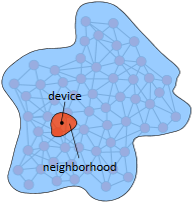
\includegraphics[width=0.2\linewidth]{imgs/dev-nei.png}
\end{frame}


\begin{frame}
\centering
\frametitle{Aggregate programming layers \small [J. Beal et al., IEEE Computer, 2015]}
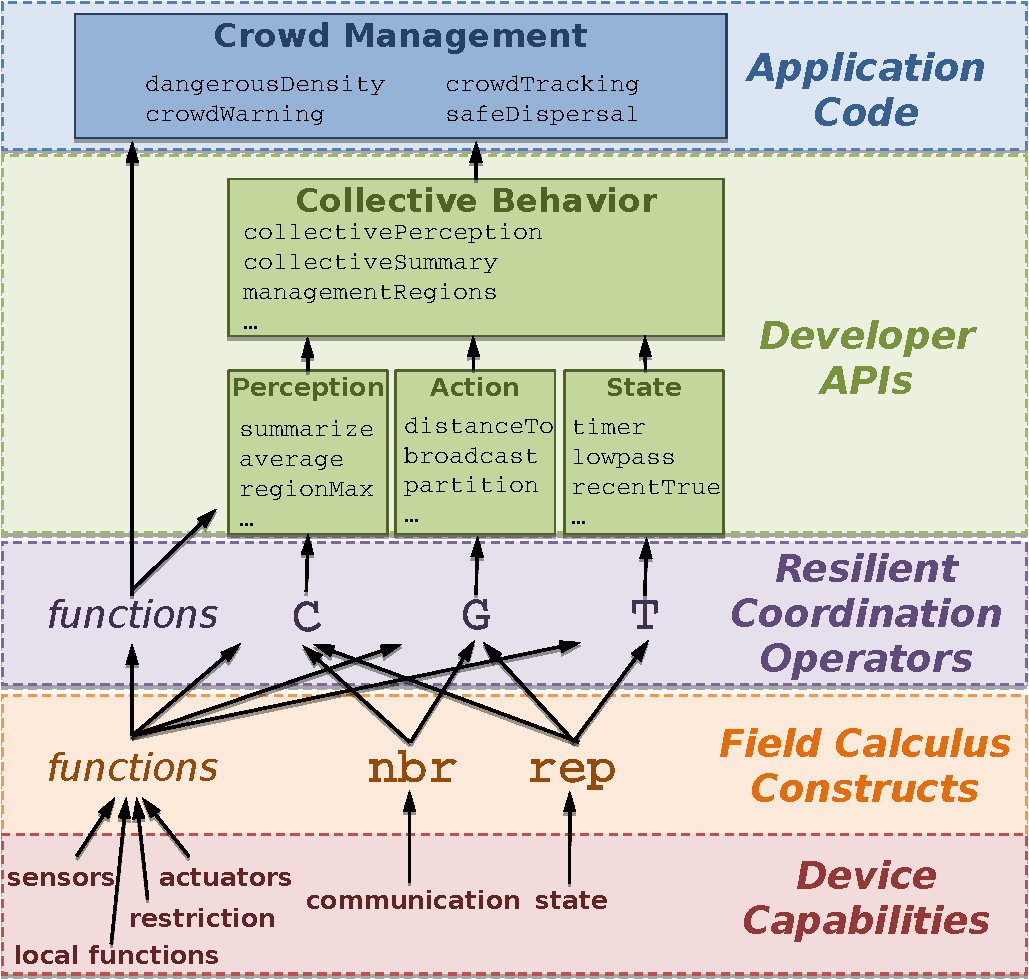
\includegraphics[height=7cm]{imgs/layers.pdf}
\end{frame}

\begin{frame}
\frametitle{Field Calculus \small [G. Audrito et al., ACM TOCL, 2019]}
\begin{block}{}
Formal language and model based on \textit{computational fields}.
\end{block}
\begin{block}{Syntax}
\centering
\centerline{\scalebox{0.9}{$
        \begin{array}{lcl@{\hspace{18mm}}r}
                \PROGRAM & \BNFcce & \overline{\FUNCTION}  \; \e
                &{ \mbox{\footnotesize program}}
                \\[3pt]
                \FUNCTION & \BNFcce &  {\color{blue} \defK} \,\; \fname (\overline{\xname}) \; \{ \e \}
                &{ \mbox{\footnotesize function declaration}}
                \\[3pt]
                \e & \BNFcce &  \xname \;\BNFmid\; \anyvalue \;\BNFmid\;  (\overline{\xname}) \toSym{\name} \e \; \BNFmid \; \e(\overline\e) \;\BNFmid\;  &{ \mbox{\footnotesize expression}} \\
                && {\color{red} \nbrK}\{\e\} \;\BNFmid\; {\color{red} \repK}(\e)\{ (\xname) \ftoSym \e \} \; \BNFmid \; \\
                && {\color{red} \shareK}(\e)\{(\xname) \ftoSym \e \} \;\BNFmid \; \\
                && {\color{red} \fifK} (\e) \{\e\} {\color{red} \elseK} \{\e\} 
                \\[3pt]
                \anyvalue & \BNFcce &  \lvalue \; \BNFmid \; \fvalue
                &{ \mbox{\footnotesize value}}
                \\[3pt]
              \lvalue & \BNFcce &  \dcOf{\dc}{\overline\lvalue} \; \BNFmid \; \funvalue
                &{ \mbox{\footnotesize local value}}
                \\[3pt]
                \fvalue & \BNFcce &  \envmap{\overline\deviceId}{\overline\lvalue}
                &{ \mbox{\footnotesize neighbouring field value}}
                \\[3pt]
                \funvalue & \BNFcce &  \fname \; \BNFmid \; \bname \;\BNFmid\; (\overline{\xname}) \toSym{\name} \e 
                &{ \mbox{\footnotesize function value}}
                \\[3pt]
        \end{array}
        $}
}
\end{block}
\end{frame}


\begin{frame}[fragile]
\frametitle{Field Calculus \small  [G. Audrito et al., ACM TOCL, 2019]}
	\begin{block}{Example (Distribute version of Bellman-Ford algorithm)}
\begin{lstlisting}[]
def distanceTo(source) {
  rep (infinity) { (d) =>
    mux (source, 0, minHood(nbr{d} + nbrDist()))
  }
}
distanceTo(temperature() > 10)
\end{lstlisting}
\end{block}
\medskip
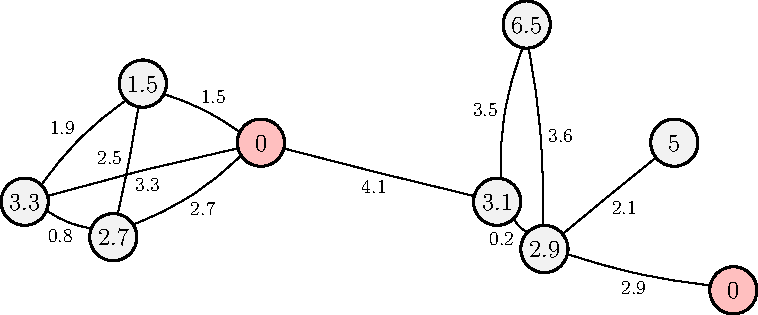
\includegraphics[width=0.65\linewidth]{imgs/gradient.pdf}
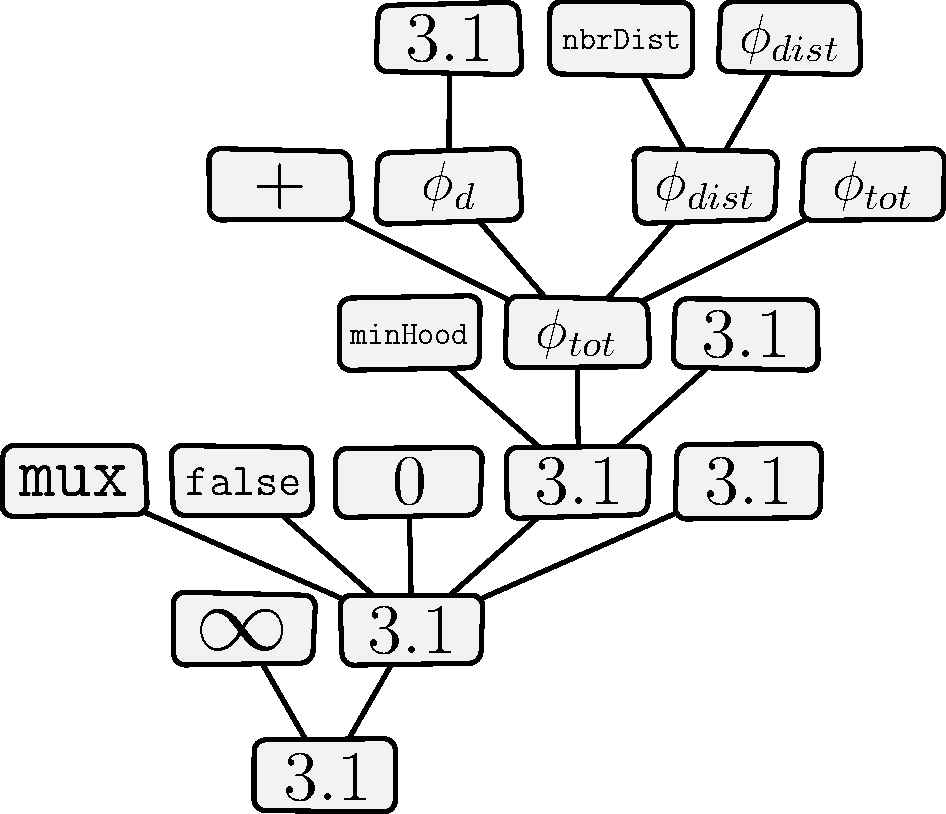
\includegraphics[width=0.3\linewidth]{imgs/valuetree.pdf}
\end{frame}

\begin{frame}
\frametitle{Goals and contributions}
\begin{block}{Goal}
Library for aggregate programming in Kotlin (\Kotac{})
\end{block}
\begin{block}{Contributions}
\begin{itemize}
\item \Kotac{} framework API and partial implementation
\item Semantics and typing formalization (\FKotac{})
\end{itemize}
\end{block}
\end{frame}

\begin{frame}[fragile]
\frametitle{Existing aggregate frameworks}
\begin{block}{Protelis \small [D. Pianini et al., ACM SAC'15] (https://protelis.github.io/)}
\begin{multicols}{2}
{Features:
\begin{itemize}
\item Java interoperability
\item Rich standard library
\item Simulation with Alchemist
\end{itemize}
}
{Limitations:
\begin{itemize}
\item External DSL
\item No typing
\item[\vspace{\fill}]
\end{itemize}
}
\end{multicols}
\end{block}
\begin{block}{Protelis example}
\begin{lstlisting}[language={Protelis}]
def distanceTo(source) {
  rep(d <- Infinity) {
    mux (source) { 0 }
    else { minHood(nbr(d) + nbrRange) }
  }
}
distanceTo(temperature() > 10)
\end{lstlisting}
\end{block}
\end{frame}

\begin{frame}[fragile]
\frametitle{Existing aggregate frameworks}
\begin{block}{\Scafi [R. Casadei, PhD Thesis 2020] (https://scafi.github.io/)}
\begin{multicols}{2}
{Features:
\begin{itemize}
\item Internal DSL in Scala
\item Expressive type-safe API
\item Akka integration
\end{itemize}
}
{Limitations:
\begin{itemize}
\item No field calculus semantics (computation against a neighbour)
\item[\vspace{\fill}]
\end{itemize}
}
\end{multicols}
\end{block}
\begin{block}{\Scafi example}
\begin{lstlisting}[language={scafi}]
def distanceTo(source: Boolean): Double {
  rep (Double.PositiveInfinity) { distance =>
     mux (source) {
        0.0
     }{
        foldhood(Double.PositiveInfinity)(Math.min){ 
          nbr{distance} /*: Double */  + nbrRange /*: Double */
        } /*: Double */
    }
  }
}
override def main() = distanceTo(temperature() > 10)
\end{lstlisting}
\end{block}
\end{frame}

\begin{frame}[fragile]
\frametitle{\Kotac}
\begin{block}{}
New aggregate programming framework for Kotlin.
\begin{itemize}
\item Internal DSL
\item Explicit fields in the type-system
\item Idiomatic Kotlin API
\item Cross-platform
\item Field calculus semantics
\end{itemize}
\end{block}
\end{frame}

\begin{frame}[fragile]
\frametitle{\Kotac}
\begin{block}{Operators API}
\begin{lstlisting}[language={kotac}]
interface AggregateContext {
    fun <T> share(initial: T, f: (Field<T>) -> T): T
    fun <K, T> align(key: K, proc: (K) -> T): T
    fun <T> nbr(f: () -> T): Field<T>
    fun <T> rep(initial: T, f: (T) -> T): T
}
\end{lstlisting}
\end{block}
\begin{block}{Example}
\begin{lstlisting}[language={kotac}]
fun AggregateContext.distanceTo(source: Boolean): Double =
  rep(Double.POSITIVE_INFINITY) { distance ->
    mux(source, 0.0, 
      (nbr { distance } /*: Field<Double> */ + 
        nbrRange /* Field<Double> */).min() /*: Double */
    )
  }
fun AggregateContext.main(): Double = distanceTo(temperature() > 10)
\end{lstlisting}
\end{block}
\end{frame}

\begin{frame}
\frametitle{\FKotac{} (Featherweight \Kotac{})}
\begin{block}{Syntax}
\centering
\centerline{\scalebox{0.85}{$
\begin{array}{l@{\hspace{1mm}}c@{\hspace{1mm}}l@{\hspace{-8mm}}r}
        \PROGRAM & \BNFcce & \overline{\FUNCTION} \; \aexp
                                                                                                                                                                                                        &   {\footnotesize \mbox{program}} \\[3pt]
        \FUNCTION & \BNFcce &  \SFUNCTION \, \BNFmid \, \AFUNCTION
                                                                                                                                                                                                        &   {\footnotesize \mbox{function declaration}} \\[3pt]
        \hline \\[-6pt]
        \SFUNCTION & \BNFcce &  \funK \; \sfname (\overline{\xname}) \; \{ \sexp \}
                                                                                                                                                                                                        &   {\footnotesize \mbox{standard function declaration}} \\[3pt]
        \sexp & \BNFcce & \xname \, \BNFmid \, \sanyvalue \, \BNFmid \, (\overline{\xname}) \; \ftoSym \{ \sexp \} \, \BNFmid \, \sexp(\overline{\sexp})
                                                                                                                                                                                                        &   {\footnotesize \mbox{standard expression}} \\[3pt]
                \sanyvalue & \BNFcce &  \lvalue \; \BNFmid \; \sfunvalue
                &{ \mbox{\footnotesize standard value}}
                \\[3pt]
                \lvalue & \BNFcce &  \dcOf{\dc}{\overline\lvalue}
                &{ \mbox{\footnotesize local data value}}
                \\[3pt]
        \sfunvalue & \BNFcce & \sbname \; \BNFmid \; \sfname \; \BNFmid \; (\overline{\xname}) \; \ftoSym \{ \sexp \}
                                                                                                                                                                                                        &   {\footnotesize\mbox{standard function value}} \\
        \hline \\[-6pt]
        \AFUNCTION & \BNFcce &  \funK \; \afname (\overline{\xname}) \; \{ \alignK{\{\aexp\}} \}
                                                                                                                                                                                                        &   {\footnotesize \mbox{aggregate function declaration}} \\[3pt]
        \aexp & \BNFcce & \xname \, \BNFmid \, \anyvalue  \BNFmid \; (\overline{\xname}) \; \toSym{\color{red}{\name}\color{black}}{\{\alignK\{\aexp\}\}} \, \BNFmid \, \aexp(\overline{\aexp}) \, \BNFmid \,  &   {\footnotesize \mbox{aggregate expression}} \\
        && \repK(\aexp)\{ (\xname) \ftoSym \aexp \} \, \BNFmid \, \nbrK\{\aexp\} \, \BNFmid \, \shareK(\aexp)\{(\xname) \ftoSym \aexp \} \\[3pt]
                \anyvalue & \BNFcce &  \lvalue \; \BNFmid \; \funvalue \; \BNFmid \; {\color{red} \fvalue}
                &{ \mbox{\footnotesize value}}
                \\[3pt]
              \funvalue & \BNFcce &  \sfunvalue \; \BNFmid \; \afunvalue
                &{ \mbox{\footnotesize function value}}
                \\[3pt]
                {\color{red} \fvalue} & \BNFcce &  {\color{red} \envmap{\overline\deviceId}{\overline\lvalue}}
                &{ \mbox{\footnotesize neighbouring field value}} \\
        \afunvalue & \BNFcce & \abname \; \BNFmid \; \afname \; \BNFmid \; (\overline{\xname}) \; \toSym{\color{red}{\name}\color{black}}{\{\alignK\{\aexp\}\}}
                                                                                                                                                                                                        &   {\footnotesize\mbox{aggregate function value}} \\
\end{array}
        $}
}
\end{block}
\end{frame}

\begin{frame}
\frametitle{\FKotac}
\begin{block}{Operational Semantics (1)}
 \scalebox{0.75}{
 $\begin{array}{l}
 \textbf{Value-trees and value-tree environments:}\\
\begin{array}{lcl@{\hspace{6.8cm}}r}
%
\vtree & \BNFcce &  \mkvt{\anyvalue}{\overline{\vtree}}    &   {\footnotesize \mbox{value-tree}} \\
\Trees & \BNFcce & \envmap{\overline{\deviceId}}{\overline{\vtree}}   &   {\footnotesize \mbox{value-tree environment}}
%
\end{array}\\[10pt]
\hline\\[-8pt]
%%%%  AUX
\textbf{Auxiliary functions:}\\
\begin{array}{l}
\begin{array}{l@{\hspace{1cm}}l}
%
\vrootOf{\mkvt{\anyvalue}{\overline{\vtree}}}  =   \anyvalue
\\
\vroot^\funvalue(\mkvt{\anyvalue}{\overline{\vtree}})  = \mkvt{\anyvalue}{} \text{ if } \funvalue \text{ standard else } \mkvt{\anyvalue}{\overline{\vtree}}
\\
%
\piIof{i}{\mkvt{\anyvalue}{\vtree_1,\ldots,\vtree_n}}  =   \vtree_i
\quad \mbox{if} \; 1\le i \le n
\\
\piBof{\funvalue}{\mkvt{\anyvalue}{\vtree_0,\ldots,\vtree_{n+1}}}  =   \vtree_{n+1}
\quad \mbox{if} \; \nameOf(\vrootOf{\vtree_{0}}) = \nameOf(\funvalue) \text{ and } \funvalue \text{ not standard}
\\
 \piBof{\funvalue}{\vtree}  =   \emptyseq \quad \mbox{otherwise}
\\  
\end{array}
\\
\mbox{For } \auxNAME\in\rho,\piI{i},\piB{\funvalue}:
\quad 
\left\{\begin{array}{lcll}
 \aux{\envmap{\deviceId}{\vtree}, \Trees}  & =  & \envmap{\deviceId}{\aux{\vtree}}, \aux{\Trees} & \quad \mbox{if} \; \aux{\vtree} \not=\emptyseq  
\\
\aux{\envmap{\deviceId}{\vtree}, \Trees}  & =   & \aux{\Trees} & \quad \mbox{if} \; \aux{\vtree}=\emptyseq  
\\
\aux{\emptyseq}  & =  &  \emptyseq
\end{array}\right.   
\\
\begin{array}{ll}
\nameOf(\fname) = \fname \qquad \nameOf(\bname) = \bname
&
\nameOf((\overline{\xname}) \; \toSym{\name}{\{\alignK\{\e\}\}}) = \name
\\
\args{\fname} = \overline{\xname} \quad \mbox{if } \, \funK \; \fname (\overline{\xname}) \; \{ \alignK{\{\e\}} \}
&
\args{\fname} = \overline{\xname} \quad \mbox{if } \, \funK \; \fname (\overline{\xname}) \; \{ \e \}
\\
\args{(\overline{\xname}) \; \toSym{\name}{\{\alignK\{\e\}\}}} = \overline{\xname}
&
\args{(\overline{\xname}) \; \ftoSym \{ \e \}} = \overline{\xname}
\\
\body{\fname} = \e  \quad \mbox{if } \, \funK \; \fname (\overline{\xname}) \; \{ \alignK{\{\e\}} \}
&
\body{\fname} = \e  \quad \mbox{if } \,  \funK \; \fname (\overline{\xname}) \; \{ \e \}
\\
\body{(\overline{\xname}) \; \toSym{\name}{\{\alignK\{\e\}\}}} = \e
&
\body{(\overline{\xname}) \; \ftoSym \{ \e \}} = \e
\end{array}
\\
\begin{array}{l@{\hspace{0.4cm}}l}
		\fvalue_0[\fvalue_1] = \fvalue_2 \; \text{ where } \fvalue_2(\deviceId) = \left\lbrace \begin{array}{ll}
			\fvalue_1(\deviceId) & \text{if } \deviceId \in \domof{\fvalue_1} \\
			\fvalue_0(\deviceId) & \text{otherwise}
		\end{array} \right. \\
\end{array}
\end{array}\\
\end{array}$
}
\end{block}
\end{frame}

\begin{frame}
\frametitle{\FKotac}
\begin{block}{Operational Semantics (2)}
 \scalebox{0.85}{
 $\begin{array}{l}
\textbf{Syntactic shorthands:}\\
\begin{array}{l@{\hspace{5pt}}l@{\hspace{5pt}}l}
\bsopsem{\deviceId}{\piIofOv{\Trees}}{\senstate}{\overline{\e}}{\overline{\vtree}}
&
  \textrm{where~~} |\overline{\e}|=n
&
  \textrm{for~~}
  \bsopsem{\deviceId}{\piIof{1}{\Trees}}{\senstate}{\e_1}{\vtree_1}
    \cdots
    \bsopsem{\deviceId}{\piIof{n}{\Trees}}{\senstate}{\e_n}{\vtree_n} \!\!\!\!\!\!\!\!\!\!\!\! \\
\vrootOf{\overline{\vtree}}
&
  \textrm{where~~} |\overline{\vtree}|=n
  & \textrm{for~~}
\vrootOf{\vtree_1},\ldots,\vrootOf{\vtree_n}\\
\substitution{\overline{\xname}}{\vrootOf{\overline{\vtree}}}
&   \textrm{where~~} |\overline{\xname}|=n
  &
  \textrm{for~~}
\substitution{\xname_1}{\vrootOf{\vtree_1}}~\ldots\quad\substitution{\xname_n}{\vrootOf{\vtree_n}}
\end{array}\\
\hline\\[-10pt]
%%%  EVALUATION RULES
\textbf{Rules for expression evaluation:} \hspace{4.4cm} %\hfill
%\vspace{-0.2cm}
  \boxed{\bsopsem{\deviceId}{\Trees}{\senstate}{\e}{\vtree}}
\skiptransition%[-5pt]
\begin{array}{c}
%\vspace{-0.1cm}
\surfaceTyping{E-LOC}{
	\e = \lvalue \text{ or } \funvalue
}{
	\bsopsem{\deviceId}{\Trees}{\senstate}{\e}{\mkvt{\e}{}}
}
\qquad\qquad
\surfaceTyping{E-FLD}{\qquad \fvalue' = \proj{\fvalue}{\domof{\Trees}\cup\{\deviceId\}}}{
\bsopsem{\deviceId}{\Trees}{\senstate}{\fvalue}{\mkvt{\fvalue'}{}}
}
\skiptransition\\[-6pt]
\surfaceTyping{E-B-APP}{  \quad
\begin{array}{c}
  \bsopsem{\deviceId}{\piIofOv{\Trees}}{\senstate}{\overline{\e},\e}{\overline{\vtree},\vtree}
  \qquad \bname = \vrootOf{\vtree}
  \qquad \vtree'=\builtinop{\bname}{\correction{\deviceId}}{\piBof{\bname}{\Trees},\senstate}(\vrootOf{\overline{\vtree}})
\end{array}
 }{
\bsopsem{\deviceId}{\Trees}{\senstate}{\e(\overline{\e})}{\mkvt{\vrootOf{\vtree'}}{\vtree,\overline{\vtree},\vroot^\bname(\vtree')}}
}
%
\skiptransition\\[-6pt]
%
\surfaceTyping{E-D-APP}{ \quad
\begin{array}{c}
  \bsopsem{\deviceId}{\piIofOv{\Trees}}{\senstate}{\overline{\e},\e}{\overline{\vtree},\vtree} \qquad 
  \funvalue=\vrootOf{\vtree} \mbox{ not a built-in} \qquad
\\
  \bsopsem{\deviceId}{\piBof{\funvalue}{\Trees}}{\senstate}{\applySubstitution{\body{\funvalue}}{\substitution{\args{\funvalue}}{\vrootOf{\overline{\vtree}}}}}{\vtree'}
\end{array}
}{
\bsopsem{\deviceId}{\Trees}{\senstate}{\e(\overline{\e})}{\mkvt{\vrootOf{\vtree'}}{\vtree,\overline{\vtree},\vroot^\funvalue(\vtree')}}
}
\end{array}
\end{array}$
}
\end{block}
\end{frame}

\begin{frame}
\frametitle{\FKotac}
\begin{block}{Operational Semantics (3)}
 \scalebox{0.85}{
 $\begin{array}{l}
%%%  EVALUATION RULES
\textbf{Rules for expression evaluation:} \hspace{4.4cm} %\hfill
%\vspace{-0.2cm}
  \boxed{\bsopsem{\deviceId}{\Trees}{\senstate}{\e}{\vtree}}
\skiptransition%[-5pt]
\begin{array}{c}
\surfaceTyping{E-NBR}{
         \qquad
     \Trees_1=\piIof{1}{\Trees} \qquad
     \bsopsem{\deviceId}{\Trees_1}{\senstate}{\e}{\vtree_1}
\qquad
 \fvalue=\mapupdate{\vrootOf{\Trees_1}}{\envmap{\deviceId}{\vrootOf{\vtree_1}}}
 }{
\bsopsem{\deviceId}{\Trees}{\senstate}{\nbrK\{\e\}}{\mkvt{\fvalue}{\vtree_1}}
}
\skiptransition\\[-6pt]
\surfaceTyping{E-REP}{
        \quad
        \begin{array}{l}
     \bsopsem{\deviceId}{\piIof{1}{\Trees}}{\senstate}{\e_1}{\vtree_1} \\
     \bsopsem{\deviceId}{\piIof{2}{\Trees}}{\senstate}{\applySubstitution{\e_2}{\substitution{\xname}{\lvalue_0}}}{\vtree_2}~~
        \end{array}
        \quad
        \lvalue_0 \! = \!\left\{\begin{array}{ll}
                             \vrootOf{\piIof{2}{\Trees}}(\deviceId) & \mbox{if} \;  \deviceId \in \domof{\Trees} \\
                             \vrootOf{\vtree_{1}} & \mbox{otherwise}
                           \end{array}\right.
 }{
\bsopsem{\deviceId}{\Trees}{\senstate}{\repK(\e_1)\{(\xname) \; \ftoSym \; \e_2\}}{\mkvt{\vrootOf{\vtree_{2}}}{\vtree_1,\vtree_2}}
}
\skiptransition\\[-4pt]
\surfaceTyping{E-SHARE}{ \qquad
	\begin{array}{l@{\hspace{0.5em}}l}
     \bsopsem{\deviceId}{\piIof{1}{\Trees}}{{\senstate}}{\e_1}{\vtree_1} & \fvalue' = \vrootOf{\piIof{2}{\Trees}} 
      \qquad \qquad \fvalue = (\envmap{\deviceId}{\vrootOf{\vtree_1}})[\fvalue']
     \\
     \bsopsem{\deviceId}{\piIof{2}{\Trees}}{{\senstate}}{\applySubstitution{\e_2}{\substitution{\xname}{\fvalue}}}{\vtree_2} %& \fvalue = (\envmap{\deviceId}{\vrootOf{\vtree_1}})[\fvalue']
	\end{array}
	\!\!\!\!
 }{
	\bsopsem{\deviceId}{\Trees}{\senstate}{\shareK(\e_1)\{(\xname) \; \ftoSym \; \e_2\}}{\mkvt{\vrootOf{\vtree_{2}}}{\vtree_1,\vtree_2}}
}
\end{array}
\end{array}$
}
\end{block}
\end{frame}

\begin{frame}
\frametitle{\FKotac}
\begin{block}{Typing (1)}
\centering
 \scalebox{0.8}{
 $\begin{array}{l}
%%%  TYPES
\textbf{Types:}\\
\begin{array}{rcl@{\hspace{4.5cm}}r}
\type & \BNFcce &  \tvar  \; \BNFmid \;  \builtintype \; \BNFmid \;  (\overline\type) \rightarrow \type  \; \BNFmid \; \ftypeOf{\builtintype}       &   {\footnotesize \mbox{type}} \\
%
\builtintype & \BNFcce & \bvar\; \BNFmid \;  \bitype &   {\footnotesize \mbox{built-in type}} \\
%
\typescheme & \BNFcce &  \forall\overline{\tvar}\overline{\bvar}.\type      &   {\footnotesize \mbox{type scheme}} \\
%
\hline\\[-8pt]
\tctx & \BNFcce &  \aann \; \BNFmid \;  \sann &   {\footnotesize \mbox{context}} \\[8pt]
%
%\localenv & \BNFcce & \envS{\senstate}{\overline\vtree} &   {\footnotesize \mbox{local environment}} \\
\end{array}\\
\hline\\[-8pt]
%%%  TYPE RULES
\textbf{Expression typing:} 
  \hfill
  \boxed{\expTypJudC{\tctx}{\TStypEnv}{\TtypEnv}{\e}{\type}}
\vspace{0.1cm}
  \\
\begin{array}{c}
\surfaceTyping{T-ATOS}{ \quad
\expTypJudC{\aann}{\TStypEnv}{\TtypEnv}{\e}{\builtintype}
}{
\expTypJudC{\sann}{\TStypEnv}{\TtypEnv}{\e}{\builtintype}
}
\qquad
\surfaceTyping{T-STOA}{ \quad
\expTypJudC{\sann}{\TStypEnv}{\TtypEnv}{\e}{\builtintype}
}{
\expTypJudC{\aann}{\TStypEnv}{\TtypEnv}{\e}{\builtintype}
}
\skiptransition
%
\nullsurfaceTyping{T-VAR}{
\expTypJudC{\tctx}{\TStypEnv}{\TtypEnv,\xname:\type}{\xname}{\type}
}
\skiptransition
%
{
\surfaceTyping{T-DAT}{ \quad
\applySubstitution{\applySubstitution{\type'}{\substitution{\overline\tvar}{\overline\type''}}}{\substitution{\overline\bvar}{\overline\builtintype}} = (\overline{\type})\rightarrow\type
\qquad
\expTypJudC{\tctx}{\TStypEnv}{\TtypEnv}{\overline{\lvalue}}{\overline{\type}}
}{
\expTypJudC{\tctx}{\TStypEnv,\dc: \forall \overline{\tvar}\overline{\bvar}. \type'}{\TtypEnv}{\dc(\overline{\lvalue})}{\type} }
}
\end{array}
\end{array}$}
\end{block}
\end{frame}

\begin{frame}
\frametitle{\FKotac}
\begin{block}{Typing (2)}
 \scalebox{0.8}{
 $\begin{array}{l}
\textbf{Expression typing:} 
  \hfill
  \boxed{\expTypJudC{\tctx}{\TStypEnv}{\TtypEnv}{\e}{\type}}
\vspace{0.1cm}
  \\
\begin{array}{c}
\surfaceTyping{T-A-AFUN}{ \quad
\expTypJudC{\aann}{\TStypEnv}{\;\TtypEnv,\,\overline{\xname}:\overline{\type}}{\e}{\type}
}{ \expTypJudC{\aann}{\TStypEnv}{\TtypEnv}{ (\overline{\xname}) \; \toSym{\name}{\{\alignK\{\e\}\}}}{(\overline{\type})\rightarrow\type}}
%
\skiptransition
%
\surfaceTyping{T-A-SFUN}{ \quad
\expTypJudC{\sann}{\TStypEnv}{\;\TtypEnv,\,\overline{\xname}:\overline{\type}}{\e}{\type}
}{ \expTypJudC{\sann}{\TStypEnv}{\TtypEnv}{ (\overline{\xname}) \; \ftoSym \{\e\}}{(\overline{\type})\rightarrow\type}}
%
\skiptransition
%
{
\surfaceTyping{T-N-AFUN}{ \quad
\mbox{$\afunvalue$ is a (built-in or declared) aggregate function}}{
\expTypJudC{\aann}{\TStypEnv,\afunvalue: \forall \overline{\tvar}\overline{\bvar}. \type}{\TtypEnv}{\afunvalue}{\applySubstitution{\applySubstitution{\type}{\substitution{\overline\tvar}{\overline\type}}}}{\substitution{\overline\bvar}{\overline\builtintype}} }
}
%
\skiptransition
%
{
\surfaceTyping{T-N-SFUN}{ \quad
\mbox{$\sfunvalue$ is a (built-in or declared) standard function}}{
\expTypJudC{\sann}{\TStypEnv,\sfunvalue: \forall \overline{\tvar}\overline{\bvar}. \type}{\TtypEnv}{\sfunvalue}{\applySubstitution{\applySubstitution{\type}{\substitution{\overline\tvar}{\overline\type}}}}{\substitution{\overline\bvar}{\overline\builtintype}} }
}
%
\skiptransition
%
\surfaceTyping{T-APP}{ \quad
\expTypJudC{\tctx}{\TStypEnv}{\TtypEnv}{\e}{(\overline{\type})\rightarrow\type} \qquad
\expTypJudC{\tctx}{\TStypEnv}{\TtypEnv}{\overline{\e}}{\overline{\type}} }{
\expTypJudC{\tctx}{\TStypEnv}{\TtypEnv}{\e(\overline{\e})}{\type} }
%
\skiptransition
%
%\surfaceTyping{T-BRANCH}{ \qquad
%\expTypJud{\TStypEnv}{\TtypEnv}{\e_1}{\btype}
%\quad \expTypJud{\TStypEnv}{\TtypEnv}{\e_2}{\type}
%\quad \expTypJud{\TStypEnv}{\TtypEnv}{\e_3}{\type} }{
%\expTypJud{\TStypEnv}{\TtypEnv}{\ifK(\e_1) \{\e_2\} \{\e_3\} }{\type} }
%%
%\skiptransition
%%
\surfaceTyping{T-REP}{ \qquad
\expTypJudC{\aann}{\TStypEnv}{\TtypEnv}{\e_1}{\builtintype}
\qquad \expTypJudC{\aann}{\TStypEnv}{\TtypEnv,\xname:\builtintype}{\e_2}{\builtintype} }{
\expTypJudC{\aann}{\TStypEnv}{\TtypEnv}{\repK(\e_1)\{(\xname) \ftoSym \e_2\}}{\builtintype} }
%
\qquad\qquad
%
\surfaceTyping{T-NBR}{ \qquad
\expTypJudC{\aann}{\TStypEnv}{\TtypEnv}{\e}{\builtintype}
}{ \expTypJudC{\aann}{\TStypEnv}{\TtypEnv}{\nbrK\{\e\}}{\ftypeOf{\builtintype}} }
%
\skiptransition
%
\surfaceTyping{T-SHARE}{ \qquad
\expTypJudC{\aann}{\TStypEnv}{\TtypEnv}{\e_1}{\builtintype}
\qquad \expTypJudC{\aann}{\TStypEnv}{\TtypEnv,\xname:\ftypeOf{\builtintype}}{\e_2}{\builtintype} }{
\expTypJudC{\aann}{\TStypEnv}{\TtypEnv}{\shareK(\e_1)\{(\xname) \ftoSym \e_2 \}}{\builtintype} }
%
\skiptransition
%
\end{array}
\end{array}$}
\end{block}
\end{frame}

\begin{frame}
\frametitle{\FKotac}
\begin{block}{Typing (3)}
\centering
 \scalebox{0.85}{
 $\begin{array}{l}
\textbf{Function typing:} 
  \hfill
  \boxed{\funTypJud{\TStypEnv}{\FUNCTION}{\typescheme}}
  \\
\begin{array}{c}
%
\surfaceTyping{T-AFUNCTION}{
\qquad
\expTypJudC{\aann}{\TStypEnv,\,\afname:\forall\emptyseq.(\overline{\type})\rightarrow\type}{\overline{\xname}:\overline{\type}}{\e}{\type}
\qquad
\overline{\tvar}\overline{\bvar}=\FTV{(\overline{\type})\rightarrow\type}
}{ \funTypJud{\TStypEnv}{\funK \; \afname (\overline{\xname}) \; \{ \alignK{\{\e\}} \}}{\forall\overline{\tvar}\overline{\bvar}.(\overline{\type})\rightarrow\type}}
%
\skiptransition
%
%
\surfaceTyping{T-SFUNCTION}{
\qquad
\expTypJudC{\sann}{\TStypEnv,\,\sfname:\forall\emptyseq.(\overline{\type})\rightarrow\type}{\overline{\xname}:\overline{\type}}{\e}{\type}
\qquad
\overline{\tvar}\overline{\bvar}=\FTV{(\overline{\type})\rightarrow\type}
}{ \funTypJud{\TStypEnv}{\funK \; \sfname (\overline{\xname}) \; \{ \e\}}{\forall\overline{\tvar}\overline{\bvar}.(\overline{\type})\rightarrow\type}}
%
\skiptransition
%
\end{array}
\\
\textbf{Program typing:} 
  \hfill
  \boxed{\proTypJud{\PROGRAM}{\type}}
  \\
\begin{array}{c}
%
\surfaceTyping{T-PROGRAM}{
\\
\TStypEnv_0=\OStypEnv
\\
\FUNCTION_i = \funK \; \fname_i (\_) \; \feqSymK{\_}
\qquad
\funTypJud{\TStypEnv_{i-1}}{\FUNCTION_i}{\typescheme_i}
\qquad
\TStypEnv_i=\TStypEnv_{i-1},\, \fname_i:\typescheme_i
\qquad
 (i \in 1..n)
\\
\expTypJudC{\aann}{\TStypEnv_n}{\emptyset}{\e}{\type}
}{ \proTypJud{\FUNCTION_1\cdots\FUNCTION_n  \;
\e}{\type}}
\end{array}
\end{array}$}
\end{block}
\end{frame}

\begin{frame}
\frametitle{Future works}
\begin{block}{Contributions}
\begin{itemize}
\item \Kotac{} API definition and partial implementation
\item \FKotac{} syntax, semantics and typing
\end{itemize}
\end{block}
\begin{block}{Future works}
\begin{itemize}
\item Complete formalization with proof of properties
\item Complete implementation of \Kotac{}
\item Validation on industrial applications
\end{itemize}
\end{block}
\end{frame}


\begin{frame}
\centering
\Huge Thanks
\end{frame}

\begin{frame}
\frametitle{Bibliography}
J. Beal, D. Pianini and M. Viroli (2015). Aggregate Programming for the Internet of Things. \textit{Computer}, vol. 48, no. 9, pp. 22-30, Sept. 2015, doi: 10.1109/MC.2015.261.

\medskip

M. Viroli, G. Audrito, F. Damiani, D. Pianini, and J. Beal (2019). A higher-order calculus of computational fields. \textit{ACM Transactions on Computational Logic}, 20, 10 2019.

\medskip

C. Roberto (2020). Engineering Self-Adaptive Collective Processes for Cyber-Physical Ecosystems, Dissertation thesis, Alma Mater Studiorum Università di Bologna.  Dottorato di ricerca in Computer science and engineering, 32 Ciclo. DOI 10.6092/unibo/amsdottorato/9380.

\medskip

D. Pianini, M. Viroli, J. Beal (2015). Protelis: Practical Aggregate Programming. \textit{ACM Symposium on Applied Computing 2015}, April 2015.
\end{frame}


\begin{frame}[fragile]
\frametitle{Field Calculus}
	\begin{block}{Example (Distribute version of Bellman-Ford algorithm with share operator)}
\begin{lstlisting}[]
def distanceTo(source) {
  share (infinity) { (d) =>
    mux (source, 0, minHood(d + nbrDist()))
  }
}
distanceTo(temperature() > 10)
\end{lstlisting}
\end{block}
\end{frame}

\end{document}
